%Welcome! This is Someday's XeLaTeX Template. 
%Developer: Someday(BUAA-SCSE)
%Any advice? Please contact: somedayjiayi@163.com

\documentclass{ctexart}

%********************导言区宏包引入********************
\usepackage{xeCJK}
\usepackage{amssymb}
\usepackage{amsmath}
\usepackage{listings} %代码
\usepackage{graphicx}
\usepackage{xcolor}
\usepackage{geometry} %页面设置
\usepackage{fontspec}
\usepackage{times}
\usepackage{fancyhdr} %页眉页脚
\pagestyle{fancy}
\usepackage{float} %表格位置
\usepackage{titlesec}
\usepackage[nofonts]{ctex}
%********************导言区宏包引入********************

%********************第三方字体引入********************
\setCJKmainfont[Path=fonts/,BoldFont=simhei.ttf,ItalicFont=simkai.ttf,TypeWriterFont=simfang.ttf]{simsun.ttc}
%中文字体涵盖黑体、宋体、楷体、仿宋

\setmainfont[Path=fonts/]{Times New Roman.ttf}
\setmonofont[Path=fonts/]{Courier New.tff}
%********************第三方字体引入********************


%********************中文字号设置********************
%\newcommand{\chuhao}{\fontsize{42pt}{\baselineskip}\selectfont}
\newcommand{\chuhao}{\fontsize{42pt}\selectfont}
\newcommand{\xiaochuhao}{\fontsize{36pt}\selectfont}
\newcommand{\yihao}{\fontsize{28pt}\selectfont}
\newcommand{\erhao}{\fontsize{21pt}\selectfont}
\newcommand{\xiaoerhao}{\fontsize{18pt}\selectfont}
\newcommand{\sanhao}{\fontsize{15.75pt}\selectfont}
\newcommand{\sihao}{\fontsize{14pt}\selectfont}
\newcommand{\xiaosihao}{\fontsize{12pt}\selectfont}
\newcommand{\wuhao}{\fontsize{10.5pt}\selectfont}
\newcommand{\xiaowuhao}{\fontsize{9pt}\selectfont}
\newcommand{\liuhao}{\fontsize{7.875pt}\selectfont}
\newcommand{\qihao}{\fontsize{5.25pt}\selectfont}
%********************中文字号设置********************


%********************页边距设置********************
\geometry{left=3cm,right=2.5cm,top=2.5cm,bottom=2.5cm}
%页边距
%********************页边距设置********************


%Welcome! This is Someday's XeLaTeX Template. 
%Developer: Someday(BUAA-SCSE)
%Any advice? Please contact: somedayjiayi@163.com
\begin{document}

%********************页眉页脚设置********************
\lhead{}%设置左页眉为空
\rhead{}%设置左页眉为空
%********************页眉页脚设置********************


%********************标题格式设置********************
\setcounter{secnumdepth}{0}%该命令取消了章标题前数字label
%********************标题格式设置********************

%\setcounter{section}{-3}  %标题计数器
%\stepcounter{section}




%********************封面部分********************

\includegraphics[scale=1]{include_picture/xiaohui.png}
%格式控制部分
\ \\ 
\ \\
\ \\
\begin{center}

\includegraphics[scale=1]{include_picture/xiaoming.png}
\end{center}
%格式控制部分
\ \\
\ \\
\ \\
\erhao
\centerline{\textbf{本模板由北航计算机学院Someday开发}} %黑体这样调用,其余字体同理
%格式控制部分
\ \\
\centerline{本模板供所有用户免费使用,勿做商用}
%格式控制部分
\ \\
\ \\
\ \\
\sihao
\centerline{\textbf{学院:计算机学院}}
\ \\
\centerline{\textbf{本模板作者:Someday}}
\ \\
\centerline{\textbf{联系作者:somedayjiayi@163.com}}
%格式控制部分
\ \\
\ \\ 
\ \\
\sanhao
\centerline{\textbf{二〇一七年七月}}

\pagenumbering{} %封面无页码
\renewcommand{\headrulewidth}{0pt}%没有页眉装饰线


%********************封面部分********************
%Welcome! This is Someday's XeLaTeX Template. 
%Developer: Someday(BUAA-SCSE)
%Any advice? Please contact: somedayjiayi@163.com
\clearpage

%********************摘要部分********************
\pagenumbering{roman} %摘要目录页小写罗马

\xiaosihao
\section*{摘要}
万万没想到。

\section*{Abstract}
lalalalala.
%********************摘要部分********************


%********************目录部分********************
\clearpage
\tableofcontents
\clearpage
%********************目录部分********************



\renewcommand{\headrulewidth}{0.4pt} %恢复页眉装饰线

%********************正文页眉部分********************
%\lhead{} 
\chead{本模板系北航计算机学院Someday所开发,供所有用户免费使用,勿做商用} %设置居中页眉
%********************正文页眉部分********************

\pagenumbering{arabic} %正文页码从1开始,用阿拉伯数字
\setcounter{page}{1} 


\section{第一章\ 公式和中文字体\ \ 和谐共处}

公式和中文字体和谐共处。\\

\subsection{第一节\ LaTeX公式}

%********************正文部分********************
\begin{align*}
S=\iint\limits_{\Sigma}1 \ ds &= \int_0^{\pi}d\theta \int_0^{2\pi} r^2sin(\theta) d\phi \\
&= \int_0^{\pi}d\theta \int_0^{2\pi}\sin (\theta ) \left(\frac{1}{5} \sin (\theta  m) \sin (n \phi )+1\right)^2d\phi\\
&=\frac{4 \sin (\pi  m) \sin ^2(\pi  n)}{5 n-5 m^2 n}-\frac{\left(8 m^2+\cos (2 \pi  m)-1\right) \sin (4 \pi  n)}{200 \left(4 m^2-1\right) n}+\frac{\pi  \left(8 m^2+\cos (2 \pi  m)-1\right)}{50 \left(4 m^2-1\right)}+4 \pi\\
&=  \left(\frac{8 m^2}{50 \left(4 m^2-1\right)}+4\right)\pi
\end{align*}
%********************正文部分********************

\subsection{第二节\ 中文字体设置}

默认就是宋体。\par
调用黑体:\textbf{黑体写在这里}\par
调用楷体:\textit{楷体写在这里}\par
调用仿宋:\texttt{仿宋写在这里}\par

\subsection{第三节\ 对齐方式}


%********************排版部分********************
\begin{center} 
居中文本第一行\\
居中文本第二行\\
\end{center}

\begin{flushright}
右对齐第一行\\
右对齐第二行\\
\end{flushright}

%********************排版部分********************


%Welcome! This is Someday's XeLaTeX Template. 
%Developer: Someday(BUAA-SCSE)
%Any advice? Please contact: somedayjiayi@163.com

\section{第二章\ 图片与TeX子文件\ \ 信手拈来}

图片与TeX子文件信手拈来。

\subsection{第一节\ 图片}

%********************图片部分********************
\begin{center}
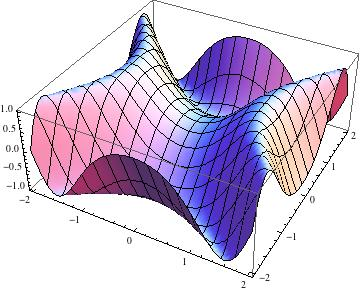
\includegraphics[scale=0.4]{include_picture/picture.jpg}\par
\end{center}
%********************图片部分********************

\subsection{第二节\ 引用Tex子文件}


%********************引用Tex子文件部分********************
*****以下内容均为引用部分*****\\
(1)解:$\because$ 根据和差化积 $\sin{\alpha}-\sin{\beta}=2\cos{\frac{\alpha+\beta}{2}}\sin{\frac{\alpha-\beta}{2}}$\\
$\therefore \sin{\sqrt{x+k}}-\sin{\sqrt{x}}=2\cos{\frac{\sqrt{x+k}+\sqrt{x}}{2}}\sin{\frac{\sqrt{x+k}-\sqrt{x}}{2}}$\\
$\therefore \lim\limits_{x \to +\infty}{\sin{\sqrt{x+k}}-\sin{\sqrt{x}}}
=\lim\limits_{x \to +\infty}{2\cos{\frac{\sqrt{x+k}+\sqrt{x}}{2}}\sin{\frac{\sqrt{x+k}-\sqrt{x}}{2}}}\\
=\lim\limits_{x \to +\infty}{cos{\frac{\sqrt{x+k}+\sqrt{x}}{2}}{\left(\sqrt{x+k}-\sqrt{x}\right)}}$\\
又$\lim\limits_{x \to +\infty}{\sqrt{x+k}-\sqrt{x}}=0,$
且$0\leqslant \left| \cos{\frac{\sqrt{x+k}+\sqrt{x}}{2}} \right|\leqslant 1$\\
$\therefore \lim\limits_{x \to +\infty}{\sin{\sqrt{x+k}}-\sin{\sqrt{x}}}
=\lim\limits_{x \to +\infty}{cos{\frac{\sqrt{x+k}+\sqrt{x}}{2}}{\left (\sqrt{x+k}-\sqrt{x}\right)}}=0$\\
(2)解:设
$$a_k=\begin{cases}
b_1-b_n &k=1,\\
b_k-b_{k-1} &2\leqslant k \leqslant n
\end{cases}$$\\
$\therefore$可以满足$\sum\limits_{k=1}^{n}{a_k}=0$,设定$b_0=b_n$\\
$\therefore \lim\limits_{x\to+\infty}{\sum\limits_{k=1}^{n}{{a_k}\sin{\sqrt{x+k}}}}
=\lim\limits_{x\to+\infty}{\sum\limits_{k=1}^{n}{{b_k-b_{k-1}}\sin{\sqrt{x+k}}}}\\
=\lim\limits_{x\to+\infty}{-\sum\limits_{k=1}^{n-1}{b_i{\left( \sin{\sqrt{x+k+1}}-\sin{\sqrt{x+k}} \right)}}-b_n{\left( \sin{\sqrt{x+1}}-\sin{\sqrt{x+k}} \right)}}$\\
又$\lim\limits_{x\to +\infty}{\sin{\sqrt{x+k}}-\sin{\sqrt{x}}}=0$\\
$\therefore \lim\limits_{x\to+\infty}{\sum\limits_{k=1}^{n}{\sin{\sqrt{x+k}}}}=0$\\
*****以上内容均为引用部分*****\\ %使用input不分页
%\include{includetex} %使用include将分页
%********************引用Tex子文件部分********************


%\titleformat*{\subsubsection}{\scshape\MakeLowercase}


\clearpage
\section{第三章\ 表格\ \ 提升逼格}

搞科研怎么能没有表格?\\

\subsection{第一节\ 表格}

%********************表格部分********************
关于表格的各种样式,请使用百度大法。\\
\begin{table}[H]
\caption{设置表格总长} 
\begin{tabular*}{12cm}{lll}
\hline  
Start & End  & Character Block Name \\  
\hline  
3400  & 4DB5 & CJK Unified Ideographs Extension A \\  
4E00  & 9FFF & CJK Unified Ideographs \\  
\hline  
\end{tabular*} 
\end{table} 
%********************表格部分********************

\section{第四章\ 未完待续}

目前该模板基本可以应付日常论文写作需要,\par
尤其是对于我航学子,你们看看这个模板,是不是似曾相识,(尤其是能不能过冯如杯格式审查)。\par
限于精力,更多高级功能,请待作者再择良辰,Someday有朝一日还会回来。

%Welcome! This is Someday's XeLaTeX Template. 
%Developer: Someday(BUAA-SCSE)
%Any advice? Please contact: somedayjiayi@163.com


%********************代码部分********************

\clearpage
\section{第五章\ 代码片\ \ 程序员的最爱}
代码片永远是程序员的最爱,支持语法高亮,用法不妨百度。\\
\lstset{language=C}
\begin{lstlisting}
#include<iostream>
using namespace std;
int main()
{
    return 0;
}
\end{lstlisting}

%********************代码部分********************


\end{document}


%Welcome! This is Someday's XeLaTeX Template. 
%Developer: Someday(BUAA-SCSE)
%Any advice? Please contact: somedayjiayi@163.com